
\def\resdir{4ethernet}

% ----------------------------------------------------------------------
\section{Ethernet}
% ----------------------------------------------------------------------

% ----------------------------------------------------------------------
\subsection{Adresse MAC}
% ----------------------------------------------------------------------

% ----------------------------------------------------------------------
\begin{frame}{Ethernet}
	\centering
	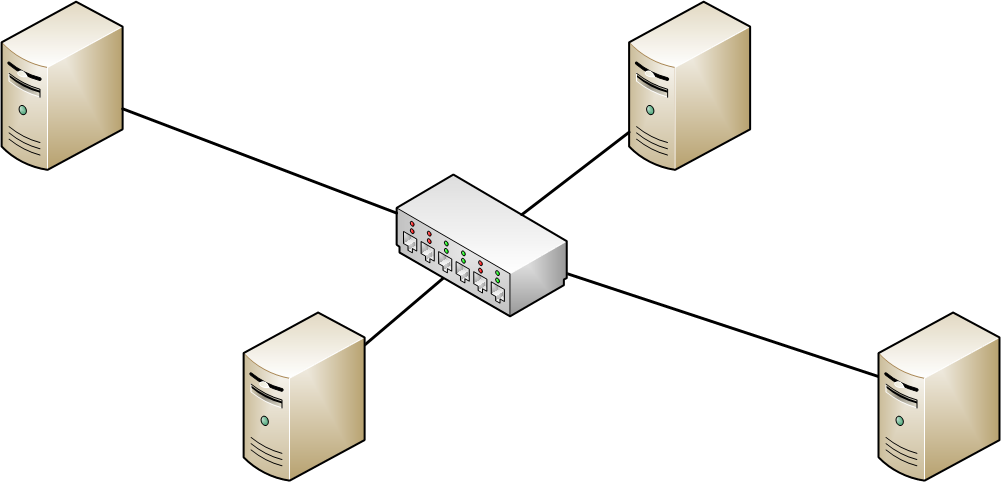
\includegraphics[height=0.4\textheight]{\resdir/etoile}
	
	\begin{block}<+-> {Ethernet - Topologie}
		\begin{itemize}
			\item En \'Etoile
			\item Autour d'un hub ou d'un switch
			\item Unique m�dium de communication
		\end{itemize}
	\end{block}
	
\end{frame}
% ----------------------------------------------------------------------

% ----------------------------------------------------------------------
\begin{frame}{\'Etoile autour d'un HUB}
	\centering
	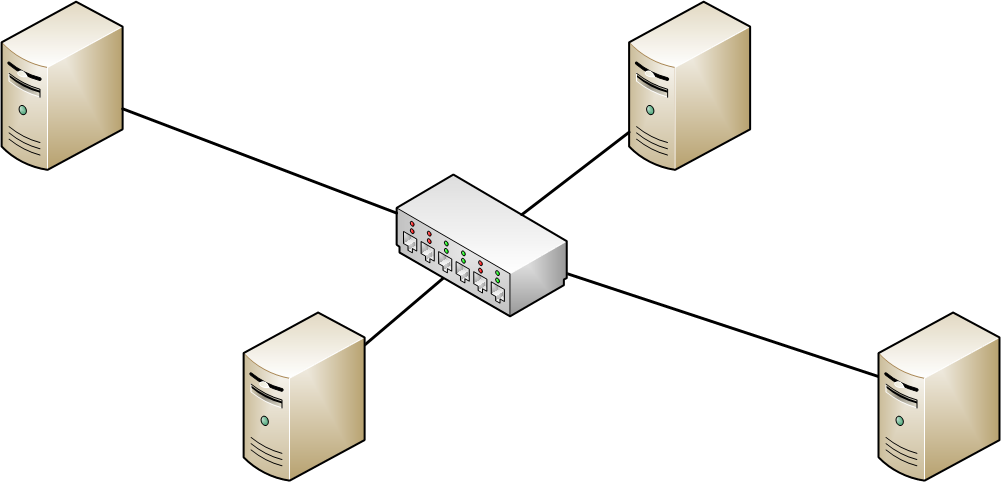
\includegraphics[height=0.6\textheight]{\resdir/etoile}
		
\end{frame}
% ----------------------------------------------------------------------
\begin{frame}{\'Etoile autour d'un HUB = BUS}
	\centering
	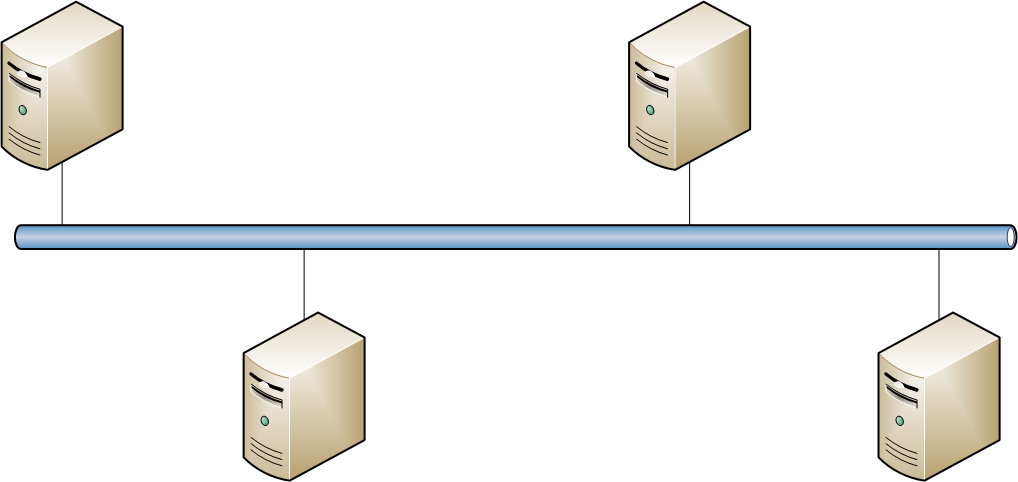
\includegraphics[height=0.6\textheight]{\resdir/bus1}
		
\end{frame}
% ----------------------------------------------------------------------
\begin{frame}{Communications montantes et descendante}
	\centering
	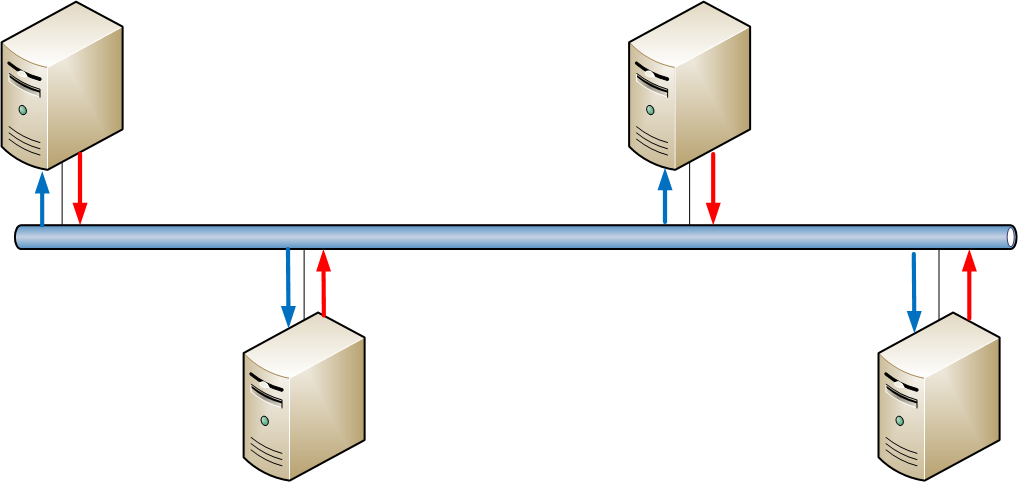
\includegraphics[height=0.6\textheight]{\resdir/bus2}
		
\end{frame}
% ----------------------------------------------------------------------
\begin{frame}{Adresse MAC (Media Access Control) pour filtrage}
	\centering
	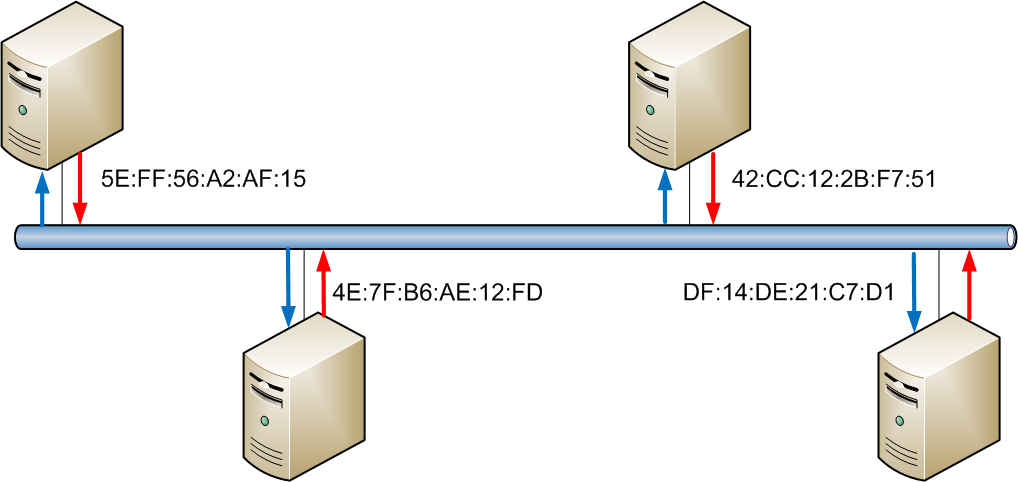
\includegraphics[height=0.6\textheight]{\resdir/busmac}
		
\end{frame}
% ----------------------------------------------------------------------

% ----------------------------------------------------------------------
\subsection{Protocole Ethernet}
% ----------------------------------------------------------------------

% ----------------------------------------------------------------------
\begin{frame}{M�dium unique = unique \textit{parleur}}
	\centering
	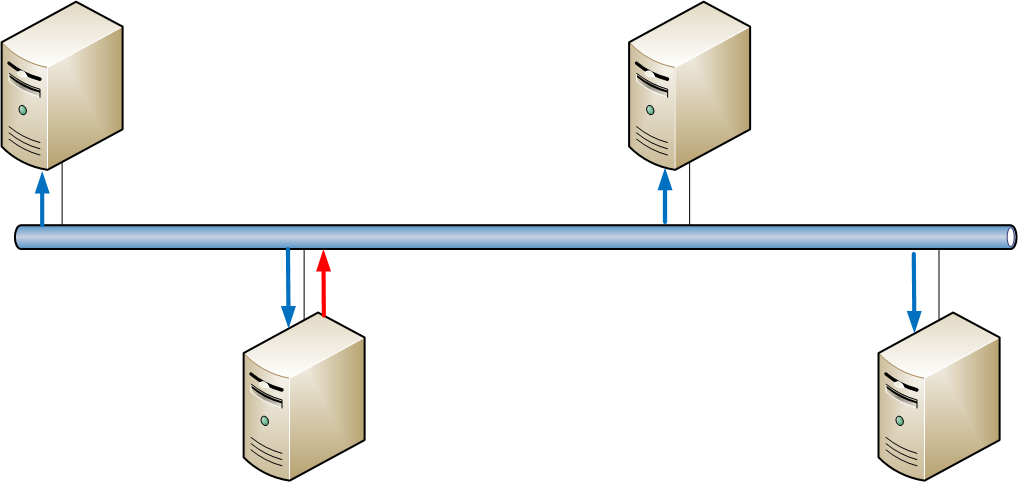
\includegraphics[height=0.6\textheight]{\resdir/bus3}
		
\end{frame}
% ----------------------------------------------------------------------
\begin{frame}{Parole � tour de r�le}
	\centering
	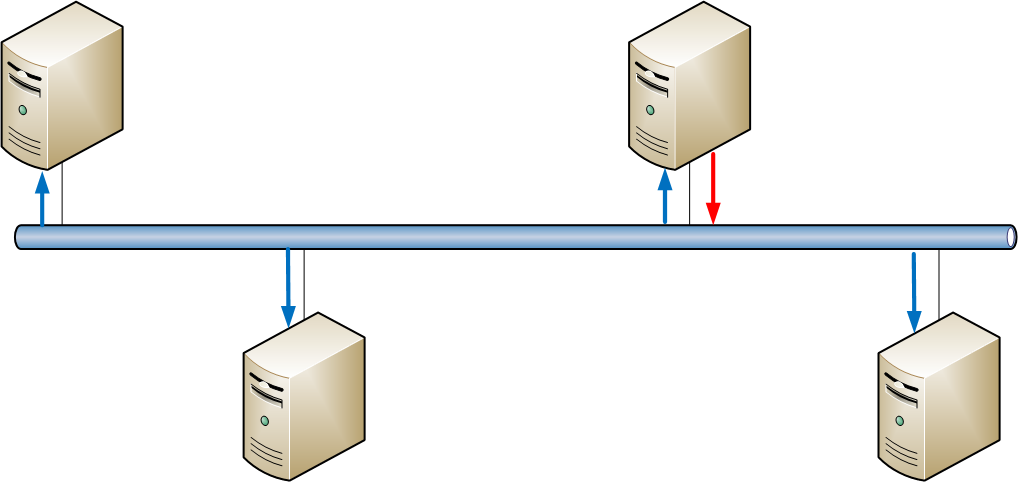
\includegraphics[height=0.6\textheight]{\resdir/bus4}
		
\end{frame}
% ----------------------------------------------------------------------


% ----------------------------------------------------------------------
\begin{frame}{Ethernet - Protocole}
	
			\small
			\begin{enumerate}
			\item \textit{d�but de transmission :} Si le m�dia n'est pas utilis�, commencer la transmission, sinon aller � l'�tape 4
			\item \textit{transmission de l'information :} Si une collision est d�tect�e, continue � transmettre jusqu'� ce que le temps minimal pour un paquet soit d�pass� (pour s'assurer que tous les postes d�tectent la collision), puis aller � l'�tape 4
			\item \textit{fin d'une transmission r�ussie :} Indiquer la r�ussite au protocole du niveau sup�rieur et sortir du mode de transfert.
			\item \textit{c�ble occup� :} Attendre jusqu'� ce que le fil soit inutilis�.
			\item \textit{le c�ble est redevenu libre :} Attendre pendant un temps al�atoire, puis retourner � l'�tape 1, sauf si le nombre maximal d'essais de transmission a �t� d�pass�.
			\item \textit{nombre maximal d'essais de transmission d�pass� :} Annoncer l'�chec au protocole de niveau sup�rieur et sortir du mode de transmission.
			\end{enumerate}
		
\end{frame}
% ----------------------------------------------------------------------


% ----------------------------------------------------------------------
\subsection{Ethernet Commut�}
% ----------------------------------------------------------------------

% ----------------------------------------------------------------------
\begin{frame}{Ethernet Commut�}

	\centering
	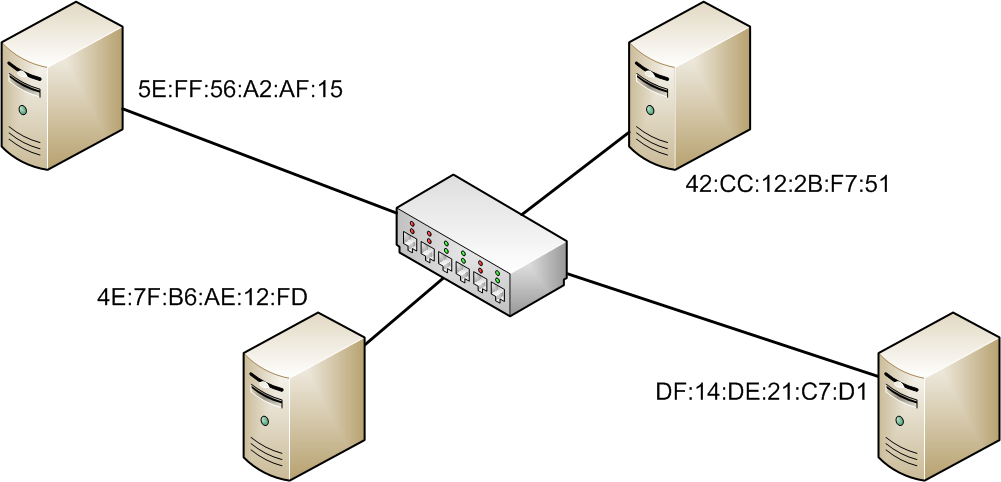
\includegraphics[height=0.6\textheight]{\resdir/switchmac}
		
			\begin{itemize}
				\item Hub vs. switch
				\item Avantage ?
				\item Comment ca marche ?
			\end{itemize}
					
\end{frame}
% ----------------------------------------------------------------------

% ----------------------------------------------------------------------
\begin{frame}{Ethernet Commut�}

	\centering
	
	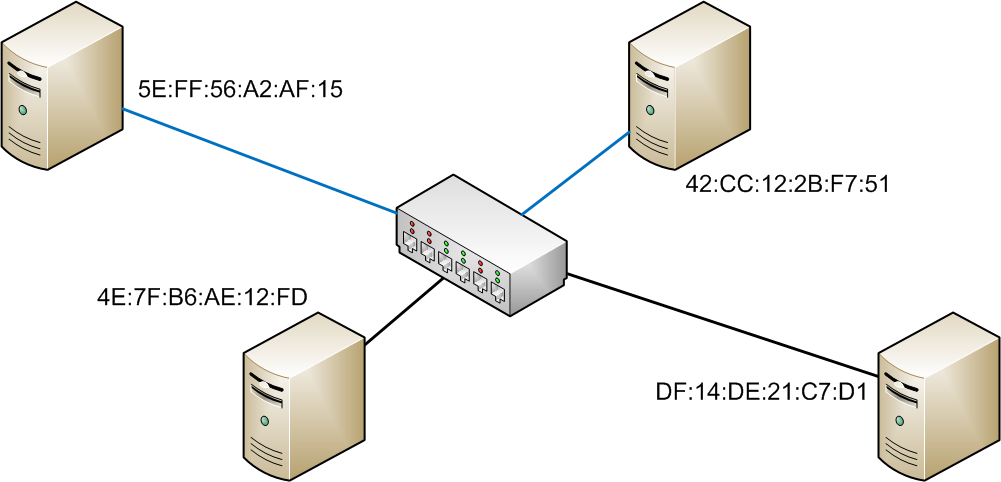
\includegraphics[height=0.6\textheight]{\resdir/switchmac1}
		
			\begin{itemize}
				\item Hub vs. switch
				\item Avantage ?
				\item Comment ca marche ?
			\end{itemize}
					
\end{frame}
% ----------------------------------------------------------------------

% ----------------------------------------------------------------------
\begin{frame}{Ethernet Commut�}

	\centering
	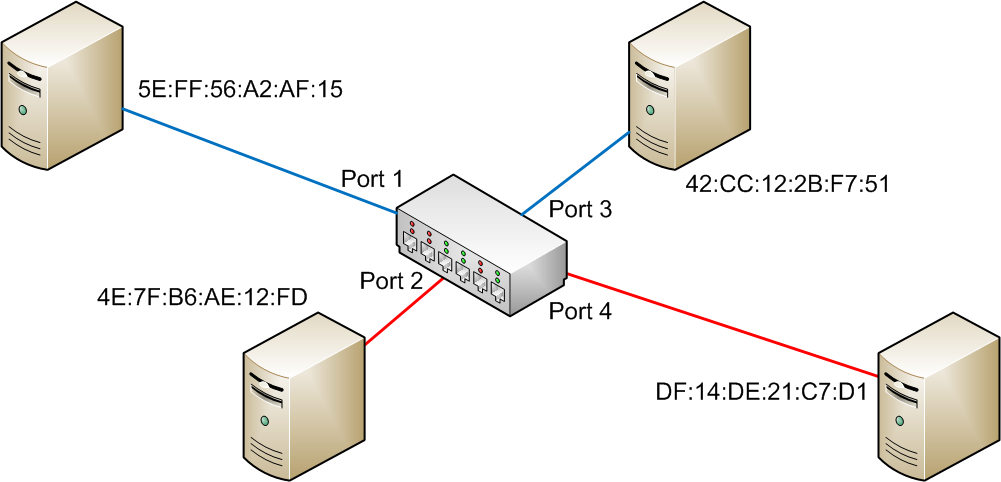
\includegraphics[height=0.6\textheight]{\resdir/switchmacport}
		
			\begin{tabular}{|c|c|}
				\hline
				MAC & Port \\
				\hline
				$5E:FF:56:A2:AF:15$ & $1$ \\ 
				$4E:7F:B6:AE:12:FD$ & $2$ \\
				$42:CC:12:2B:F7:51$ & $3$ \\
				$DF:14:DE:21:C7:D1$ & $4$ \\
				\hline
			\end{tabular}
					
\end{frame}
% ----------------------------------------------------------------------
